\setcounter{figure}{0}

\section{10th September 2023: A spousal tiff}
\subsection*{Text: Song of Solomon 5:2-6:3}
  \begin{quote}
    She

    [2] I slept, but my heart was awake.
    A sound! My beloved is knocking.
    “Open to me, my sister, my love,
        my dove, my perfect one,
    for my head is wet with dew,
        my locks with the drops of the night.”
    [3] I had put off my garment;
        how could I put it on?
    I had bathed my feet;
        how could I soil them?
    [4] My beloved put his hand to the latch,
        and my heart was thrilled within me.
    [5] I arose to open to my beloved,
        and my hands dripped with myrrh,
    my fingers with liquid myrrh,
        on the handles of the bolt.
    [6] I opened to my beloved,
        but my beloved had turned and gone.
    My soul failed me when he spoke.
    I sought him, but found him not;
        I called him, but he gave no answer.
    [7] The watchmen found me
        as they went about in the city;
    they beat me, they bruised me,
        they took away my veil,
        those watchmen of the walls.
    [8] I adjure you, O daughters of Jerusalem,
        if you find my beloved,
    that you tell him
        I am sick with love.


    Others

    [9] What is your beloved more than another beloved,
        O most beautiful among women?
    What is your beloved more than another beloved,
        that you thus adjure us?


        She

    [10] My beloved is radiant and ruddy,
        distinguished among ten thousand.
    [11] His head is the finest gold;
        his locks are wavy,
        black as a raven.
    [12] His eyes are like doves
        beside streams of water,
    bathed in milk,
        sitting beside a full pool.
    [13] His cheeks are like beds of spices,
        mounds of sweet-smelling herbs.
    His lips are lilies,
        dripping liquid myrrh.
    [14] His arms are rods of gold,
        set with jewels.
    His body is polished ivory,
        bedecked with sapphires.
    [15] His legs are alabaster columns,
        set on bases of gold.
    His appearance is like Lebanon,
        choice as the cedars.
    [16] His mouth is most sweet,
        and he is altogether desirable.
    This is my beloved and this is my friend,
        O daughters of Jerusalem.


    Others

    [1] Where has your beloved gone,
        O most beautiful among women?
    Where has your beloved turned,
        that we may seek him with you?


        She

    [2] My beloved has gone down to his garden
        to the beds of spices,
    to graze in the gardens
        and to gather lilies.
    [3] I am my beloved’s and my beloved is mine;
        he grazes among the lilies.
  \end{quote}
\subsection*{Notes}
\begin{itemize}
  \item{Up till now in the book, we had courtship and marriage and the consummation of marriage.}
  \item{Now in the book, we have married life together. Married life together is not always as rosy as the fairytales portray.}
  \item{In chapter 5:2-9, we have a tense mood. The point is captured in shakespeare’s quote: “the course of true love never did run smooth”. Here, the intimacy that the couple once shared is threatened. But though there are threats to intimacy, we must safeguard it and make it run straight.}
  \item{Here, most likely we have a spousal fight due to unmet expectations. The woman was waiting for the man to reach home (she was half asleep), but the man reached home quite late. The man expects the woman to be available for sex but the woman is now a little lazy, since the husband came home so late. But after a while, the wife relents and opens the door but then by then the husband is already quite annoyed and he left. Here, we have many instances of unmet expectations. Perhaps the wife should have communicated that she wanted the husband to come home earlier, and perhaps the husband could have communicated an apology, and etc. }
  \item{Unmet expectations can cause tensions in the marriage, so there is a need to communicate so expectations can be aligned, and the communication has to be done amicably.}
  \item{The greatest obstacle to intimacy is selfishness and self centredness. Both the woman and man are selfish here.
  \begin{itemize}
    \item{He is selfish --- he comes home so late and still expects to have sex}
    \item{She is selfish --- she is unwilling to let him in because it is inconvenient}
  \end{itemize}}
  \item{The opposite of selfishness is selflessness.}
  \item{Here, from v4 onwards, we see the woman shifting from thinking just about herself to thinking about her husband. She goes in search for her man in the city. Probably she was not literally beaten, but the watchmen beating her is probably a metaphor for how defenseless she felt without her husband.}
  \item{After a while, the woman asks the daughters of jerusalem for help to find her husband, but the daughters of jerusalem ask if this man is worth it. Then, the woman replies with many praises of the man.}
  \item{By the way, v8b-v16d form a chiasm (left as an exercise to the reader. Hint: ``daughters of Jerusalem'', ``my beloved'' ,``gold'').}
  \item{After that, the husband appears with the wife, and then the intimacy is restored.}
  \item{Self-centredness and selfishness is killing many marriages. The antidote is self denial, to put the interests of our spouse above our own interests. }
  \item{An application of the above concept is in sexual intimacy. Quite often, there is a mismatch in sexual desire between husband and wife. Suppose (for the sake of argument) that the husband has more desire than the wife for sex. 
  \begin{itemize}
    \item{The wife should be ok to have sex even if she doesn’t want to, because she wants to seek her husband’s pleasure more than her own.}
    \item{The husband should be ok to not have sex though he wants to, because he wants to seek his wife’s well being more then his own.}
    \item{If both parties are so understanding towards each other (see the two points above), they will both feel loved and intimacy will naturally come.}
    \item{The opposite of the above story is that the husband is annoyed that the wife is reluctant to have sex cause she is tired and he insists on his own way. The wife hates that and she withholds it even more not just because she is tired but now also to punish the husband for not caring about her tiredness.}
    \item{Sex is a gift of God to be enjoyed by married couples, not a weapon to be used in retaliation.}
    \item{Now, human love (the r/s between husband and wife) should point us toward divine love, to the love between Christ and the Church.}
    \item{Just like in marriage, when we commit to being Christian, we should commit to a life-long pursuit of Christ. But we can do this only because Jesus denied himself first (“yet not my will, but your will be done”) and pursued us, by voluntarily self-sacrificed and died on the cross for our sins.}
    \item{Christ is the epitome of self-denial, and He has set for us a model of what it means to deny self. }
    \item{Here, we see that as the r/s matures, the starting point changes. Comparing chapter 2:16 and chapter 6:3, in chapter 2, the starting point is our desire for the beloved, but in chapter 6, as the r/s with the beloved grows, the starting point is the beloved’s desire for us.}
    \item{Today's text also has a spiritual reading:\\
    Here, Jesus is the true husband who knocks on the doors of our hearts. By our neglect, sometimes we forget Jesus and we are lazy to open the door for him. Then we feel like we can’t feel Jesus’ presence in our life. Nothing goes in when we read the Bible, and we feel weak and helpless, like when we kenna whack by the watchmen of Jerusalem. In those times, we might think: is Jesus worth it? Then, we must remember how perfect Jesus is and how he loved us first. After which, when we open the door, unlike the husband in Song of songs who leaves, we will still find Jesus there.}
  \end{itemize}}
  % \item{\begin{figure}[H]
  %   \centering
  %   % 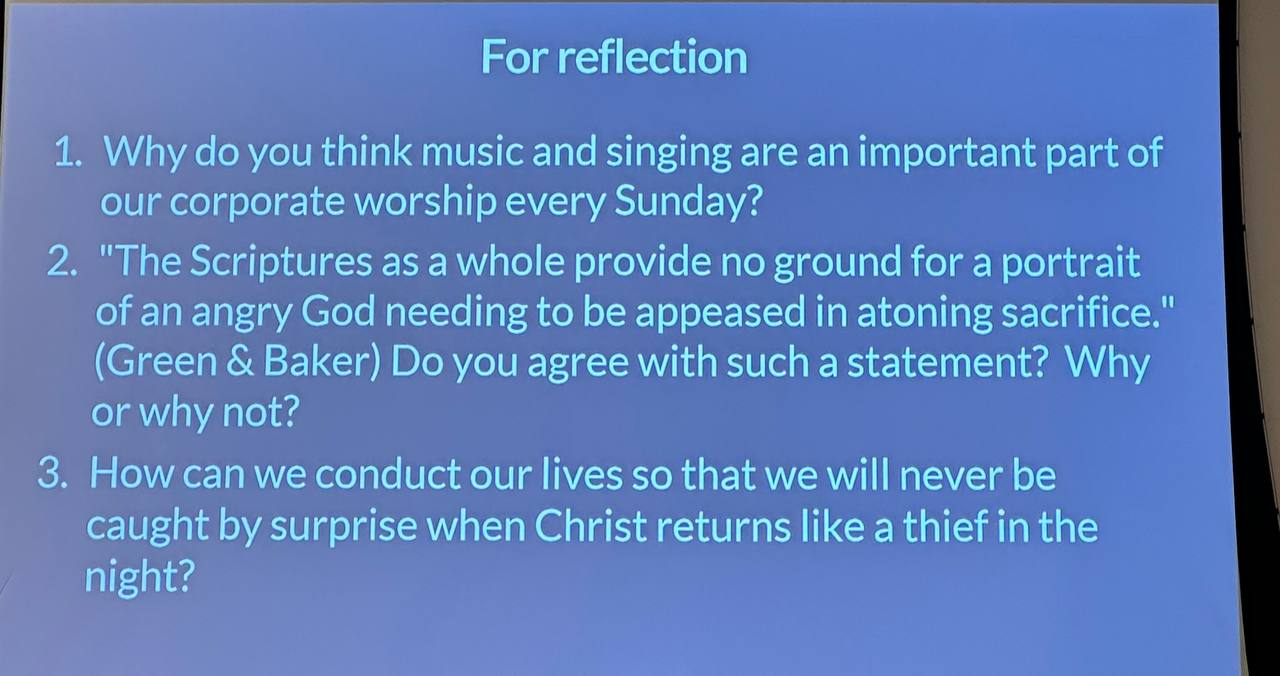
\includegraphics[width=0.8\textwidth, trim={0cm 0cm 0cm 0cm},clip]{Figures/marchSermon4Reflections.jpg}
  %   \includegraphics[width=0.8\textwidth, trim={0cm 0cm 0cm 0cm},clip]{example-image-a}
  %   \caption[]{Reflection questions for this sermon}
  %   \label{}
  % \end{figure}}
\end{itemize}